\emph{Cet exercice est un questionnaire à choix multiples.\\ Pour chacune des questions suivantes, une seule des quatre réponses proposées est exacte.\\ Pour répondre, indiquer sur la copie le numéro de la question et la lettre de la réponse choisie.\\ Aucune justification n'est demandée.\\ Une réponse fausse, une absence de réponse, ou une réponse multiple, ne rapporte ni n'enlève de point.}

\medskip

\hfill\textbf{\large L'énoncé ci-dessous est commun aux questions 1. et 2.}\hfill~

\medskip

Les 200 adhérents d’un club sont des filles ou des garçons. Ces adhérents pratiquent l'aviron ou le basket selon la répartition figurant dans le tableau ci-dessous.

\begin{center}
	\begin{tblr}{vline{1}={2-Z}{solid},vline{2-Z}={solid},hline{1}={2-Z}{solid},hline{2-Z}={solid},colspec={*{4}{Q[m,c,3cm]}}}
		 & \textbf{Aviron} & \textbf{Basket} & \textbf{Total} \\
		\textbf{Filles} & 25 & 80 & 105 \\
		\textbf{Garçon} & 50 & 45 & 95 \\
		\textbf{Total} & 75 & 125 & 200 \\
	\end{tblr}
\end{center}

On choisit un adhérent au hasard et on considère les évènements suivants
:

\smallskip

\hfill{}$F$ : l'adhérent est une fille. \hfill{}A : l'adhérent pratique l’aviron.\hfill~

\begin{enumerate}
	\item La probabilité de $F$ sachant $A$ est égale à :
	
	\medskip
	
	\begin{tblr}{width=\linewidth,colspec={*{4}{X[m,l]}}}
		\textbf{a.}~~$\frac{25}{100}$ & 
		\textbf{b.}~~$\frac{25}{75}$ & 
		\textbf{c.}~~$\frac{25}{105}$ &
		\textbf{d.}~~$\frac{75}{105}$
	\end{tblr}
	\item La probabilité de l'événement $A \cup F$ est égale à :
	
	\medskip
	
	\begin{tblr}{width=\linewidth,colspec={*{4}{X[m,l]}}}
		\textbf{a.}~~$\frac{9}{10}$ & 
		\textbf{b.}~~$\frac{1}{8}$ & 
		\textbf{c.}~~$\frac{31}{40}$ &
		\textbf{d.}~~$\frac{5}{36}$
	\end{tblr}
\end{enumerate}

\begin{center}
	$\ast\ast$
	
	\vspace*{-0.5\baselineskip}
	
	$\ast$
\end{center}

\hfill\textbf{\large L'énoncé ci-dessous est commun aux questions 3. et 4.}\hfill~

\medskip

\begin{wrapstuff}[r]
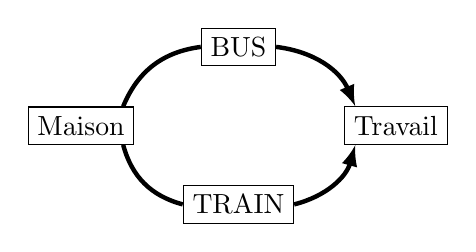
\begin{tikzpicture}
	\node[draw,rectangle] (Maison) at (0,0) {Maison} ;
	\node[draw,rectangle] (Travail) at (4,0) {Travail} ;
	\node[draw,rectangle] (BUS) at ({0.5*4},1) {BUS} ;
	\node[draw,rectangle] (TRAIN) at ({0.5*4},-1) {TRAIN} ;
	\draw[ultra thick] (BUS.west) to[bend right] ([xshift=-4pt]Maison.north east) ;
	\draw[ultra thick,->,>=latex] (BUS.east) to[bend left] ([xshift=4pt]Travail.north west) ;
	\draw[ultra thick] (TRAIN.west) to[bend left] ([xshift=-4pt]Maison.south east) ;
	\draw[ultra thick,->,>=latex] (TRAIN.east) to[bend right] ([xshift=4pt]Travail.south west) ;
\end{tikzpicture}
\end{wrapstuff}

Pour se rendre à son travail, Albert peut utiliser au choix le bus ou le train.

\smallskip

La probabilité que le bus soit en panne est égale à $b$.

La probabilité que le train soit en panne est égale à $t$.

Les pannes de bus et de train surviennent de façon indépendante.

\begin{enumerate}
	\setcounter{enumi}{2}
	\item La probabilité $p_1$, que le bus ou le train soient en panne est égale à :
	
	\medskip
	
	\begin{tblr}{width=\linewidth,colspec={*{4}{X[m,l]}}}
		\textbf{a.}~~$p_1=bt$ & 
		\textbf{b.}~~$p_1=1-bt$ & 
		\textbf{c.}~~$p_1=b+t$ &
		\textbf{d.}~~$p_1=b+t-bt$
	\end{tblr}
	\item La probabilité $p_2$ que Albert puisse se rendre à son travail est égale à :
	
	\medskip
	
	\begin{tblr}{width=\linewidth,colspec={*{4}{X[m,l]}}}
		\textbf{a.}~~$p_2=bt$ & 
		\textbf{b.}~~$p_2=1-bt$ & 
		\textbf{c.}~~$p_2=b+t$ &
		\textbf{d.}~~$p_2=b+t-bt$
	\end{tblr}
\end{enumerate}

\begin{center}
	$\ast\ast$
	
	\vspace*{-0.5\baselineskip}
	
	$\ast$
\end{center}

\begin{enumerate}[resume]
	\item On considère une pièce de monnaie pour laquelle la probabilité d'obtenir FACE est égale à $x$. On lance la pièce $n$ fois. Les lancers sont indépendants.
	
	La probabilité $p$ d'obtenir au moins une fois FACE sur les $n$ lancers est égale à :
	
	\medskip
	
	\begin{tblr}{width=\linewidth,colspec={*{4}{X[m,l]}}}
		\textbf{a.}~~$p=x^n$ & 
		\textbf{b.}~~$p=(1-x)^n$ & 
		\textbf{c.}~~$p=1-x^n$ &
		\textbf{d.}~~$p=1-(1-x)^n$
	\end{tblr}
\end{enumerate}